\chapter{磁场与带电粒子运动}

本章围绕洛伦兹力、带电粒子在磁场中的轨道、速度选择器、质谱仪以及磁约束等主题展开。基本方程为
\[
\vb*{F}=q\qty(\vb*{E}+\vb*{v}\times \vb*{B}),
\]
在纯磁场中由于磁力始终垂直于速度，故其主要作用是改变速度方向而不改变速率。

\begin{gaokao}
质量为 $m$、电荷量为 $q$ 的带电粒子以速度 $v$ 垂直射入匀强磁场，磁感应强度大小为 $B$。不计重力。
\begin{enumerate}
  \item 求粒子轨道半径；
  \item 求周期；
  \item 说明为什么磁场不改变粒子的动能。
\end{enumerate}

\begin{solution}
磁力提供向心力，故
\[
qvB=\frac{mv^2}{r}.
\]
解得轨道半径
\[
r=\frac{mv}{qB}.
\]
周期为
\[
T=\frac{2\pi r}{v}=\frac{2\pi m}{qB}.
\]
由于任意时刻
\[
\vb*{F}_B\perp \vb*{v},
\]
故磁场力做功率
\[
P=\vb*{F}_B\cdot \vb*{v}=0.
\]
既然磁场不做功，粒子速率和动能都保持不变，仅速度方向不断改变，因此轨道为圆周。
\end{solution}
\end{gaokao}

\begin{gaokao}
质谱仪中，某带电离子先经电压 $U$ 加速，再垂直进入磁感应强度为 $B$ 的分析磁场，在底片上留下半径为 $r$ 的圆弧轨迹。求该离子的比荷 $q/m$。

\begin{solution}
离子由静止加速，有
\[
qU=\frac12 mv^2.
\]
进入磁场后满足
\[
qvB=\frac{mv^2}{r}.
\]
由第二式得
\[
v=\frac{qBr}{m}.
\]
代回能量方程，得到
\[
qU=\frac12 m\qty(\frac{qBr}{m})^2=\frac{q^2B^2r^2}{2m}.
\]
故
\[
\frac{q}{m}=\frac{2U}{B^2r^2}.
\]
这正是磁偏转法测量比荷的基本原理。
\end{solution}
\end{gaokao}

\begin{gaokao}
速度选择器中，电场 $\vb*{E}$ 与磁场 $\vb*{B}$ 相互垂直，且均垂直于粒子入射速度。请从微积分与牛顿第二定律角度说明：为什么只有满足某一特定速度的粒子能沿直线通过。

\begin{center}
\begin{tikzpicture}[scale=1.0]
  \draw[->,thick] (-2,0) -- (2,0) node[right] {$\vb*{v}$};
  \draw[->,thick,blue!70!black] (0,-1.4) -- (0,1.4) node[above] {$\vb*{E}$};
  \foreach \x in {-1.4,-0.4,0.6,1.6}
    \foreach \y in {-1.0,0,1.0}
      \node at (\x,\y) {$\otimes$};
  \node at (1.7,1.3) {$\vb*{B}$ 入纸面};
\end{tikzpicture}
\end{center}

\begin{solution}
设粒子沿 $x$ 方向前进，电场沿 $y$ 方向，磁场沿 $z$ 方向，则横向受力为
\[
F_y=qE-qvB.
\]
若粒子能始终沿直线通过，必须满足横向加速度为零，即
\[
m\dv[2]{y}{t}=q(E-vB)=0.
\]
所以只有当
\[
v=\frac{E}{B}
\]
时，粒子横向净受力恒为零，轨迹保持直线。若 $v>E/B$，磁力占优，粒子向一侧偏转；若 $v<E/B$，电场力占优，粒子向另一侧偏转。微积分观点下，本质是要求横向位移函数满足 $\dv[2]{y}{t}=0$ 且初始横向速度为零。
\end{solution}
\end{gaokao}

\begin{competition}
带电粒子以速度分量 $v_\parallel$（沿磁场方向）和 $v_\perp$（垂直磁场方向）射入匀强磁场 $\vb*{B}=B\vu{z}$。建立其空间螺旋运动的参数方程。

\begin{solution}
垂直于磁场的分速度做匀速圆周运动，平行于磁场的分速度保持不变。设初始时刻粒子位于
\[
(x,y,z)=(r,0,0),
\]
且回旋角频率为
\[
\omega_c=\frac{qB}{m}.
\]
圆周半径
\[
r=\frac{mv_\perp}{qB}.
\]
于是可取参数方程
\[
x(t)=r\cos(\omega_c t),
\qquad
y(t)=r\sin(\omega_c t),
\qquad
z(t)=v_\parallel t.
\]
轨道是一条沿 $z$ 方向前进的螺旋线，其螺距为
\[
h=v_\parallel T=v_\parallel\frac{2\pi}{\omega_c}=\frac{2\pi mv_\parallel}{qB}.
\]
若 $v_\parallel=0$，退化为圆周；若 $v_\perp=0$，退化为沿磁场方向匀速直线运动。
\end{solution}
\end{competition}

\begin{competition}
在缓慢变化的非均匀磁场中，带电粒子回旋半径远小于磁场变化尺度。请定性说明磁场梯度会引起导引中心漂移，并给出漂移方向与哪些量有关。

\begin{solution}
当磁场存在空间梯度时，粒子在回旋轨道不同位置受到的磁场强弱不同，因而回旋过程中平均受力不再完全对称。这样，圆周运动的几何中心即导引中心会发生缓慢漂移，这就是梯度漂移。

对正电荷而言，若磁场方向固定而 $\nabla B$ 指向某侧，则漂移方向与
\[
\vb*{B}\times \nabla B
\]
有关；负电荷方向相反。漂移速度还与粒子的质量、垂直速度分量以及磁场强度有关。更精细地，回旋磁矩
\[
\mu=\frac{mv_\perp^2}{2B}
\]
在慢变条件下近似守恒，于是粒子会表现出“趋向磁场较弱侧”的平均动力学行为。这是磁约束物理与空间等离子体运动中的重要基础。
\end{solution}
\end{competition}

\begin{competition}
说明磁瓶约束带电粒子的基本原理：为什么粒子沿磁力线进入两端磁场增强区域后会被“反射”回来？

\begin{solution}
磁瓶中，磁场在中部较弱、两端较强。带电粒子沿磁力线运动时，若磁场变化足够缓慢，则其磁矩
\[
\mu=\frac{mv_\perp^2}{2B}
\]
近似不变。随着粒子进入两端强磁场区域，$B$ 增大，为保持 $\mu$ 近似恒定，粒子的垂直动能增加，即 $v_\perp$ 增大。

另一方面，若无外界做功，总动能
\[
\frac12 m(v_\perp^2+v_\parallel^2)
\]
守恒，因此 $v_\parallel$ 必须减小。当 $v_\parallel$ 减小到零时，粒子沿磁力线的前进停止，随后反向运动，于是被磁场“镜像反射”。只有螺旋角较小、平行速度占比太大的粒子才可能从瓶口逃逸，这构成了磁镜损失锥的概念。
\end{solution}
\end{competition}

\begin{university}
应用毕奥--萨伐尔定律说明：
\begin{enumerate}
  \item 长螺线管内部磁场为什么近似均匀；
  \item 亥姆霍兹线圈为什么能在中心区域产生高均匀度磁场。
\end{enumerate}
不要求给出冗长的闭式推导，但需写出关键积分思想。

\begin{solution}
毕奥--萨伐尔定律写为
\[
\dd{\vb*{B}}=\frac{\mu_0}{4\pi}\frac{I\dd{\vb*{l}}\times \vu{r}}{r^2}.
\]
对长螺线管，可把它视为许多圆电流环沿轴向连续叠加。轴线上各环产生的磁场方向相同，而侧向分量因对称性相消。对单位长度匝数为 $n$ 的长螺线管积分后，内部中心区域得到近似恒定的
\[
B\approx \mu_0 nI,
\]
外部则因来自不同匝的贡献大量抵消而很弱。

亥姆霍兹线圈由两个半径相同、间距等于半径的同轴圆线圈构成。中心轴线上两线圈的磁场相加后，不仅中心点的一阶导数为零，适当选取间距还能使二阶不均匀性显著减小，因此中心附近较大范围内磁场变化很小，均匀度高。这正是实验物理中常用它产生近似匀强磁场的原因。
\end{solution}
\end{university}

\begin{university}
在匀强相互垂直的电场与磁场中，推导 $\vb*{E}\times\vb*{B}$ 漂移速度，并说明其与电荷符号无关。

\begin{solution}
设磁场为 $\vb*{B}=B\vu{z}$，电场为 $\vb*{E}=E\vu{x}$。粒子满足
\[
m\dv{\vb*{v}}{t}=q(\vb*{E}+\vb*{v}\times \vb*{B}).
\]
若把速度分解为快速回旋部分与缓慢平均漂移部分，可寻找使平均受力为零的漂移速度 $\vb*{v}_d$，满足
\[
\vb*{E}+\vb*{v}_d\times \vb*{B}=0.
\]
两边叉乘 $\vb*{B}$，并利用 $\vb*{v}_d\perp \vb*{B}$，得
\[
\vb*{v}_d=\frac{\vb*{E}\times \vb*{B}}{B^2}.
\]
该式中不含 $q$，因此正负电荷具有相同的 $\vb*{E}\times\vb*{B}$ 漂移速度。物理上，这是因为不同电荷虽回旋方向相反，但在平均意义上都要寻找一个共同的平移速度，使得电场力与磁场产生的平均偏折相抵消。
\end{solution}
\end{university}

\begin{university}
简述回旋加速器的工作原理，并写出非相对论近似下回旋角频率与粒子动能随半径变化的关系。

\begin{center}
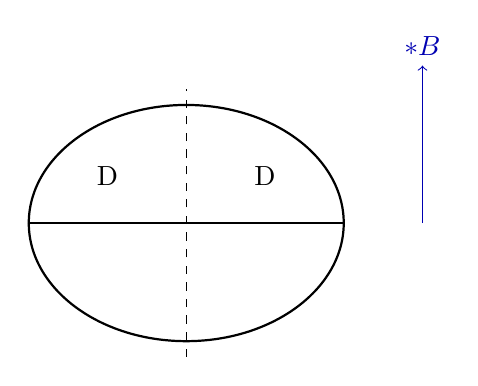
\begin{tikzpicture}[scale=1.0]
  \draw[thick] (-2,0) arc (180:0:2 and 1.5);
  \draw[thick] (-2,0) arc (180:360:2 and 1.5);
  \draw[thick] (-2,0) -- (2,0);
  \draw[dashed] (0,-1.7) -- (0,1.7);
  \node at (-1,0.6) {D};
  \node at (1,0.6) {D};
  \draw[->,blue!70!black] (3,0) -- (3,2) node[above] {$\vb*{B}$};
\end{tikzpicture}
\end{center}

\begin{solution}
回旋加速器在两个半圆形电极之间加交变电压，粒子每穿过中缝一次就被电场加速；进入电极内部后，几乎只受磁场作用而做半圆运动。非相对论条件下，回旋角频率
\[
\omega_c=\frac{qB}{m}
\]
与速度和轨道半径无关，因此只要外加交变电场频率与其同步，粒子每次过缝都能得到加速。

轨道半径满足
\[
r=\frac{mv}{qB},
\]
故随着速度增大，粒子轨道半径逐步增大，形成由内向外展开的螺旋。动能可写为
\[
K=\frac12 mv^2=\frac{q^2B^2r^2}{2m}.
\]
因此半径越大，动能越高。相对论效应显著时，由于有效质量变化，回旋频率不再恒定，这也是经典回旋加速器的限制之一。
\end{solution}
\end{university}

\begin{problem}
请定性说明磁约束聚变中托卡马克或磁镜装置试图解决的核心问题，并指出带电粒子漂移与不稳定性为何会给约束带来困难。

\begin{solution}
磁约束聚变的目标是在足够高温下把等离子体长时间限制在有限空间中，使离子与电子不会直接碰到器壁而迅速冷却。由于任何材料容器都难以承受聚变级高温，必须借助磁场来引导带电粒子运动。

困难在于：真实装置中的磁场不可能绝对均匀，粒子会发生梯度漂移、曲率漂移和 $\vb*{E}\times\vb*{B}$ 漂移；此外，等离子体还会产生宏观不稳定性、湍流与输运增强，使能量和粒子向外泄漏。于是工程上需要精心设计磁面结构、反馈控制和加热方案，以提高约束时间并满足聚变点火条件。
\end{solution}
\end{problem}

\begin{problem}
带电粒子在一般电磁场中的运动满足牛顿--洛伦兹方程。请说明为什么这一方程在很多情形下难以解析求解，以及研究者通常采用哪些近似或数值方法。

\begin{solution}
一般电磁场中，粒子满足
\[
m\dv{\vb*{v}}{t}=q\qty(\vb*{E}(\vb*{r},t)+\vb*{v}\times \vb*{B}(\vb*{r},t)),
\qquad
\dv{\vb*{r}}{t}=\vb*{v}.
\]
该方程组通常是非线性、耦合且系数随空间与时间变化的常微分方程系统，若再考虑相对论效应、辐射阻尼或自洽场，复杂度更高，因此少有简单闭式解。

常见处理办法包括：
\begin{enumerate}
  \item 在匀强场、慢变场等理想模型下求解析解；
  \item 使用导引中心近似、绝热不变量等平均方法；
  \item 对等离子体整体采用流体模型或 Vlasov 方程；
  \item 对单粒子轨道使用 Runge--Kutta、Boris 推进等数值积分算法。
\end{enumerate}
这些方法共同构成了现代等离子体物理和空间物理的基础工具箱。
\end{solution}
\end{problem}
